\chapter[Project Planning]{Project Planning}

% \section{Methodology}
% https://zube.io/blog/agile-project-management-workflow-for-github-issues/
\section{Introduction}
The project was to develop a front-end to an existing system and had to be planned accordingly. This chapter will give an overview about which parts of the whole system are already provided for and identifies the requirements and potential solutions for the frontend. Additionally, it depicts considered technologies and techniques and evaluates the most appropriate development stack.

The main idea is to give tenants, proprietors and facility management a way to communicate over a single point of access. In its first version, they should be able to discuss topics they care about, easily make announcements, submit and track the state of maintenance issues and create polls in order to provide an easy way for decision-making. The frontend is to be designed as a \acrfull{mvp} rather than adhering to exact requirements, meaning deviations are desired if it is sensible (Example found in chapter (Not yet written) ). It is noteworthy to mention that this project will initially be realeased in Austria.

% Talk about project idea in more detail
\section{Provided Services}
% DB - postgresql
% API - documented with postman
The Database and API are both provided by the project partner. The first is a PostgreSQL instance, the latter an API built on top of Django and Django Rest Framework. These two technologies provide the backend of the system as a whole. The API is documented with Postman, describing each endpoint in terms of what type of data has to be sent and what data will be returned. Apart from making these compatible with a containerized environment (see \autoref{ch:deployment}), no further action has to be taken in order to use these services.

\section{Requirements}
% List requirements defined by project partner
% write these as user stories
% illustrate as Use Case diagram
As mentioned in the introduction, several functional requirements exist. Furthermore, there are some non-functional requirements for the project which have to be taken into account. \autoref{tab:requirements} depicts these general requirements. \newline

\begin{table}[H]
    \begin{center}
      \begin{tabular}{l|l} % <-- Alignments: 1st column left, 2nd middle and 3rd right, with vertical lines in between
        \textbf{Functional Requirements} & \textbf{Non-Functional Requirements}\\
        \hline
        Digital Noticeboard & High Flexibility \\
        Polls & Easy to maintain\\
        Forum & Easy way of creating apps for mobile phones from frontend\\
        Issue Management & Low learning curve for future developers\\
        Bilinguality & \\
        Custom Authentication & \\
      \end{tabular}
      \caption{Project Requirements}
      \label{tab:requirements}
    \end{center}
  \end{table}

  
\subsection{Digital Noticeboard}
The digital noticeboard is a unidirectional way of communication between house parties. A typical example would be to announce a get-together everyone is invited to. \newline
Allowed user roles: Proprietors, Tenants, Facility Managament

\subsection{Polls}
Polls are intended to remove the friction of decision-making. An example would be a facade that has to be repainted with a new color. To get an initial idea which color it should be, Proprietors can create polls and let other proprietors choose between given options. \newline
Allowed user roles: Proprietors

\subsection{Forum}
The Forum is a way of discussing topics related to a specific house. E.g. a tenant wants to know when garbage cans are emptied. Proprietors as well as facility management and other tenants can answer such questions. \newline
Allowed user roles: Proprietors, Tenants, Facility Managament

\subsection{Issue Management}
With an issue management system, tenants or proprietors can submit and track the status of maintenance related issues. The facility management can access these issues and take action. When an issue's state changes, they can mark it accordingly in the system. \newline
Allowed user roles: Proprietors, Tenants, Facility Managament

\subsection{Bilinguality}
It is important that users are able to choose between at least two languages. German is the most obvious choice as it is Austria's primarily spoken language. English, the second most well known language in Austria is obvious as well.

\subsection{Authentication}
Users shall be authenticated via a custom endpoint defined in the API. Authentication-providers such as Google or Facebook are not needed. \newline

According to these requirements, a use-case diagram as illustrated in \autoref{fig:usecases} can be generated.
\begin{figure}[H]
    \begin{center}
    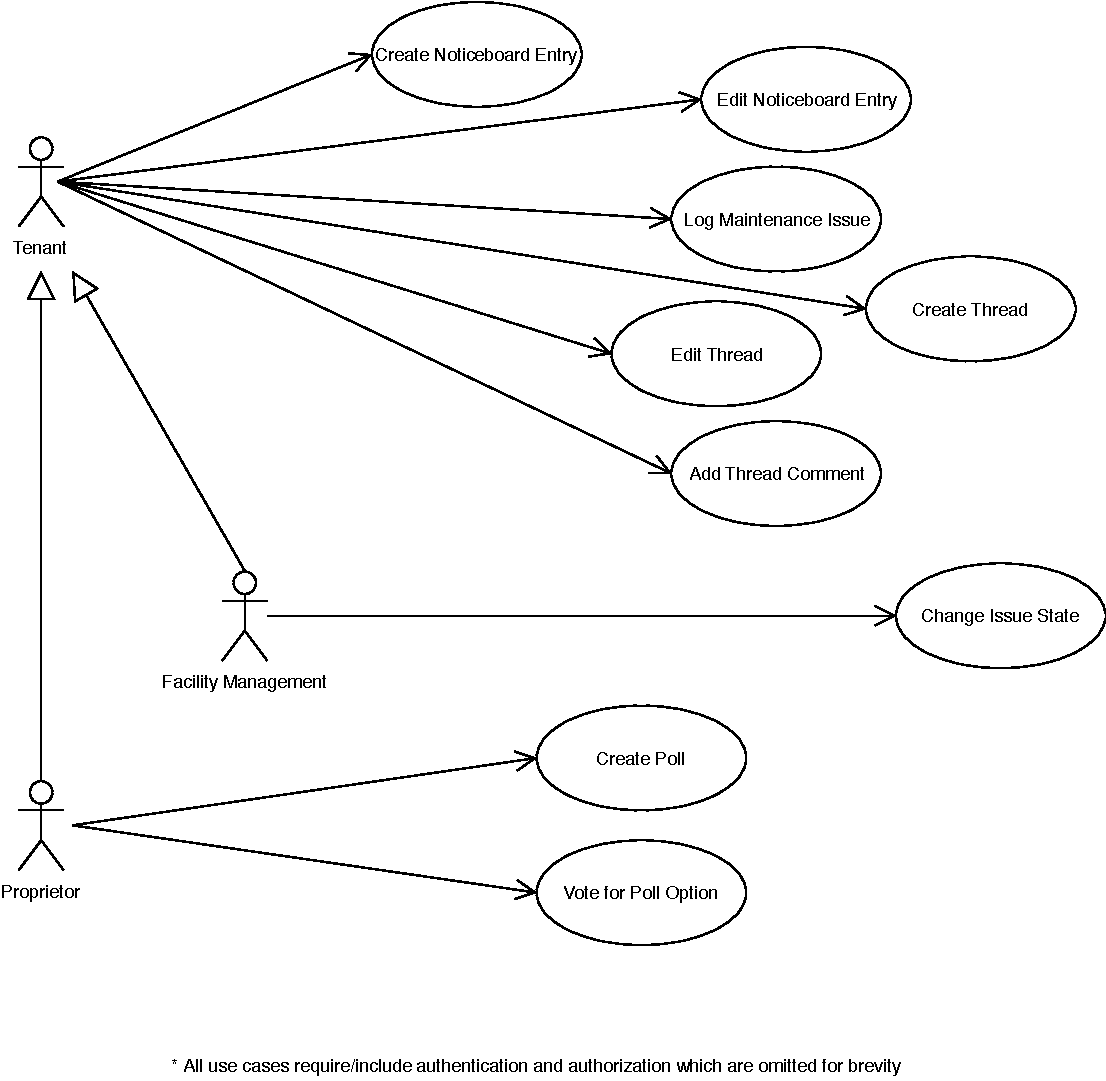
\includegraphics[height=6in,width=6in]{usecases2}
    \end{center}
    \caption{Proprietors Assembly Use Cases}
    \label{fig:usecases}
\end{figure}

\section{Considered Technologies}
% Single Page Application because interactive and functionality easy to integrate, smooth native-like feeling
% Using Vue because flexibility and ease of learning were important
\subsection{\acrshort{spa} Framework}
To meet both functional and non-functional requirements a \acrfull{spa} is a potential solution. They provide an interactive, smooth native-like user interface and can easily be transformed to a \acrfull{pwa} if the need arises. \acrshort{pwa}' are a fairly new type of application that use traditional web-browser technology but can be run almost as if they are native applications. As illustrated in \autoref{fig:comparison}, an especially appropriate framework can be found in Vue, which perfectly suits the needs of the non-functional requirements for this project. Its relatively high flexibility in addition to its shallow learning curve allow for a rapid development process.

\subsection{\acrshort{ssr} Framework}
Although the project's requirements do not state any need for \acrfull{ssr} it is possible that rapidly changing content such as publicly available blog posts with comments will be added in a future release. \autoref{subsub:seo} identifies three ways of rendering \acrshort{spa}'s on the server side and why this is useful. Server Side Rendering would be the most viable option as it comes with the biggest advantages. 

It can be utilized in one of two ways: By using vue as a framework and the supporting library "vue-server-renderer" or by using an additional framework. The first way requires the developer to configure everything themselves whereas the latter provides pre-configured \acrshort{ssr} functionality. One of these frameworks is Nuxt.js which is the most  popular SSR framework within the vue community. In addition, it configures automatic routing and state management, which are described in more detail in chapter (Not yet written) . 

\subsection{CSS Framework}
% Bulma, vuetify, bootstrap, foundation
CSS frameworks can drastically decrease developing time for frontend projects as they provide predefined tools and components for creating user interfaces. There are various CSS frameworks available which differ greatly in design: in addition to the widely used Bootstrap and Foundation frameworks which have a very basic and familiar design, there are smaller ones which provide different design elements which could help distinguish the project from others. Such frameworks are "Bulma" or "Materialize". Bulma comes with a very distinct design, that does not seem to be used as widely on the web. Furthermore, the vue library "Buefy" builds on top of Bulma's CSS and provides predefined vue components to use. This is very important as it makes it much easier and quicker to build user interfaces.

\subsection{Deployment}
There are various techniques of deploying a technology stack to a production ready environment ranging from installing a webserver, database and additional services directly onto a server (monolith) to using virtual machines for each individual service. A much better and future-proof approach is the usage of "containers": Each service is encapsulated in its own linux environment but hosted on the same machine. It is important to note that some services are bundled together in the same container if it makes sense: E.g a backend framework which defines REST endpoints and a webserver which exposes these endpoints. A more appropriate word in this case is "microservice". The most popular containerization technology is Docker which gives developers the ability to write "compose" files that define a composition of services. One of the biggest advantages of Docker is that the same services can be run in a development as well as production environment, greatly reducing overhead.

\subsection{Summary}
Vue is the perfect framework for this project due to its flexibility and ease of learning. Nuxt will be used to lay the groundwork for \acrshort{ssr}. The design of the frontend will be based on Bulma and Buefy giving the project a distinct and distinguishable look. Docker will provide a way of easily deploying the application on any server and development environment.

\section{Additional Tools and Techniques}
\subsubsection{GitLab}
GitLab not only serves as a Git-based \acrfull{vcs} but also as a container registry. The registry exposes an interface for uploading and downloading container images. This is especially useful for creating images on a local machine, uploading them to the registry and downloading them again onto a remote server where they should be deployed. Doing it this way completely removes the need of storing the source code for the whole project on the remote server and building it from source. Instead, the version number of the used image is increased in a compose file and the container gets updated accordingly when a redeployment is initiated.

\subsubsection{Git Flow}
Git Flow is a VCS methodology which is based around "features". In its most basic structure there is one master and develop branch accompanied by multiple feature branches (usually one feature per branch). The master branch should always be kept in a production-ready state, wheras the develop branch contains the actively developed project-source in which every finished feature branch is merged into. Additionally there are hotfix and release branches which support the others. Git Flow adds an abstraction layer to the development flow and greatly helps building applications by an iterative approach.

\subsubsection{Circle CI}
Automated testing is important when developing applications. It can reassure the developer that nothing will break and result in unexpected errors. Circle CI is a continuous integration platform which automatically tests code when certain rules are met. It works very well when used in addition to Git Flow and Docker: it can be set up to create a container with the projects source, builds it and runs its tests upon every change made to the develop or master branch or a pull request. Circle CI notifies its users if any step during this process failed preventing faulty code to ever reach a production state.

\section{Legal and Ethical Issues}
As identified in the Technical Report (see Appendix ...) there are two main areas of concern regarding ethical and legal issues: privacy and visual impairment. In order to use the service, users have to provide information about them, including name, email and home address which could lead to GDPR related issues. Providing access to the service to visually impaired users also poses an ethical issue as adaptions have to be carefully thought about.